\begin{frame}{Contribution 3: Proposed Models}
    \begin{block}{Objective}
        Propose new preprocessing methodologies and deep learning architectures for BP monitoring.
        Evaluate our models against reproduced models for a concrete clinical context.
    \end{block}
\end{frame}

\begin{frame}{Contribution 3: Proposed Models}{Methodology}
    Compare popular feature-extraction layers
    \begin{itemize}
        \item MLP
        \item RNN-MLP
        \item Residual CNN
        \item Transformer Encoder
    \end{itemize}

    \begin{itemize}
        \item Hyperparameter optimization
        \item Test different types of feature extraction layers
    \end{itemize}
\end{frame}

\begin{frame}{Contribution 3: Proposed Models}{MLP}
    \begin{columns}
        \column{0.5\columnwidth}
        \begin{figure}
            \includesvg[width=0.8\columnwidth]{models/MLP.svg}
        \end{figure}

        \column{0.5\columnwidth}
        \begin{itemize}
            \item 128 units hidden
            \item 2 units output
        \end{itemize}
        \begin{itemize}
            \item simplest model
        \end{itemize}
    \end{columns}

\end{frame}

\begin{frame}{Contribution 3: Proposed Models}{RNN-MLP}
    \begin{columns}
        \column{0.5\columnwidth}
        \begin{figure}
            \includesvg[width=0.8\columnwidth]{models/RNN-MLP.svg}
        \end{figure}

        \column{0.5\columnwidth}
        \begin{itemize}
            \item 256 units GRU layers
            \item stacked MLP
        \end{itemize}
    \end{columns}
\end{frame}

\begin{frame}{Contribution 3: Proposed Models}{Residual CNN}
    \begin{columns}
        \column{0.5\columnwidth}
        \begin{figure}
            \includesvg[width=0.27\columnwidth]{models/Residual Conv.svg}
            \includesvg[width=0.27\columnwidth]{models/Residual Conv - Residual Block.svg}
        \end{figure}

        \column{0.5\columnwidth}
        \begin{itemize}
            \item kernel: 3
            \item Stacked MLP with Dropout 0.01
        \end{itemize}
        \begin{tabular}{lSS}
            \hline
            Module & {Blocks} & {Filters} \\
            \hline
            1st    & 2        & 64        \\
            2nd    & 4        & 128       \\
            3rd    & 8        & 256       \\
            4th    & 2        & 256       \\
            \hline
        \end{tabular}
    \end{columns}

\end{frame}

\begin{frame}{Contribution 3: Proposed Models}{Transformer Encoder}
    \begin{columns}
        \column{0.5\columnwidth}
        \begin{figure}
            \includesvg[width=0.3\columnwidth]{models/Transformer Encoder.svg}
        \end{figure}

        \column{0.5\columnwidth}
        \begin{itemize}
            \item Encoder part only
            \item 4 attention heads
            \item First dense layer: 64 units
            \item Second dense layer: embedding size
        \end{itemize}
    \end{columns}


\end{frame}\begin{frame}{Contribution 3: Input Methodologies}{Methodology}
    Compare Input Methodologies
    \begin{itemize}
        \item Window
        \item Heartbeat
        \item Heartbeat sequence
    \end{itemize}
\end{frame}

\begin{frame}{Contribution 3: Heartbeat Sequence Input}{Methodology}
    Keep fined-grained analysis and temporal aspect
    \begin{figure}
        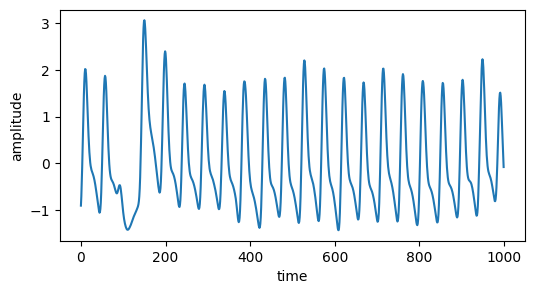
\includegraphics[width=0.35\columnwidth]{inputs/window.png}

        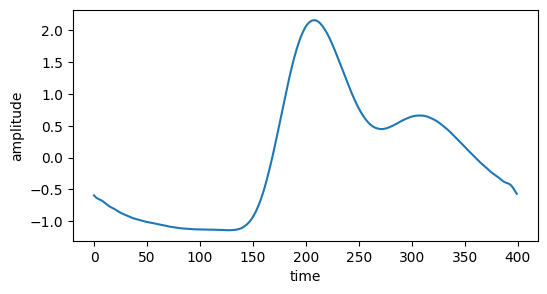
\includegraphics[width=0.35\columnwidth]{inputs/heartbeat.png}
        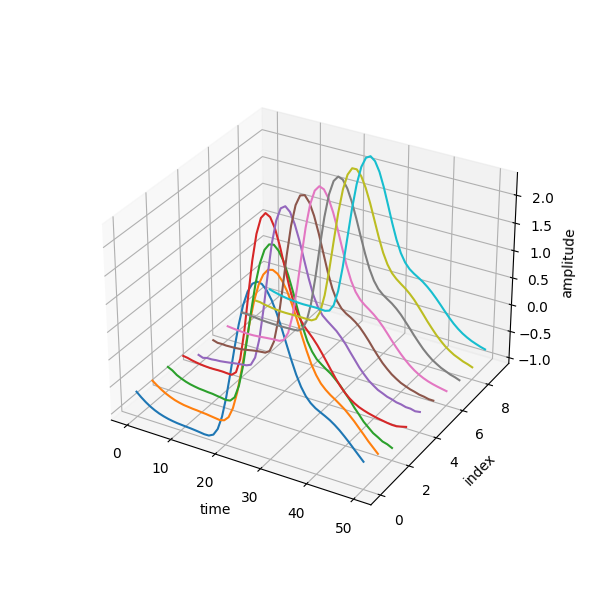
\includegraphics[width=0.35\columnwidth]{inputs/heartbeat-sequence.png}
    \end{figure}
\end{frame}


\begin{frame}{Contribution 2 \& 3}{Results}
    \centering
    Window
    \begin{figure}
        \includesvg[width=0.49\columnwidth]{results/window SBP.svg}
        \hfill
        \includesvg[width=0.49\columnwidth]{results/window DBP.svg}
    \end{figure}
    \begin{itemize}
        \item large gap between random and patient-wise split
        \item 13.802mmHg lower for random split on average
    \end{itemize}
\end{frame}

\begin{frame}{Contribution 2 \& 3}{Results}
    \centering
    Heartbeat
    \begin{figure}
        \includesvg[width=0.49\columnwidth]{results/heartbeat SBP.svg}
        \hfill
        \includesvg[width=0.49\columnwidth]{results/heartbeat DBP.svg}
    \end{figure}
    \begin{itemize}
        \item Random split is most often used in the literature
    \end{itemize}
\end{frame}


\begin{frame}{Contribution 2 \& 3}{Results}
    \centering
    Heartbeat Sequence
    \begin{figure}
        \includesvg[width=0.49\columnwidth]{results/beatsequence SBP.svg}
        \hfill
        \includesvg[width=0.49\columnwidth]{results/beatsequence DBP.svg}
    \end{figure}
    \begin{itemize}
        \item Random split passes AAMI, but does not generalize
        \item No models meet AAMI standard for patient-wise
    \end{itemize}
\end{frame}

\begin{frame}{Contribution 2 \& 3}{Results}
    \centering
    Heartbeat Sequence
    \begin{figure}
        \includesvg[width=0.49\columnwidth]{results/beatsequence SBP.svg}
        \hfill
        \includesvg[width=0.49\columnwidth]{results/beatsequence DBP.svg}
    \end{figure}
    \begin{itemize}
        \item Random split passes AAMI, but does not generalize
        \item No models meet AAMI standard for patient-wise
    \end{itemize}
\end{frame}

\begin{frame}{Contribution 2 \& 3}{Results}
    \begin{block}{Main Finding \#1}
        Non-invasive, calibration-free BP monitoring remains an unsolved problem.
    \end{block}
\end{frame}

\begin{frame}{Contribution 2 \& 3}{Results}
    \begin{columns}
        \column{0.5\columnwidth}
        \centering
        Best patient-wise
        \begin{figure}
            \includesvg[height=0.3\textheight]{models/MLP.svg}
        \end{figure}

        \begin{table}[htbp]
            \centering
            \resizebox{\linewidth}{!}{
                \begin{tabular}{SSSS}
                    \hline
                    \multicolumn{2}{c}{SBP (mmHg)} & \multicolumn{2}{c}{DBP (mmHg)}                  \\
                    \cmidrule(lr){1-2} \cmidrule(lr){3-4}
                    {MAE}                          & {SD}                           & {MAE}  & {SD}  \\
                    \hline
                    18.547                         & 14.054                         & 10.152 & 6.986 \\
                    \hline
                \end{tabular}
            }
        \end{table}

        \column{0.5\columnwidth}
        \centering
        Best overall
        \begin{figure}
            \includesvg[height=0.3\textheight]{models/RNN-MLP.svg}
        \end{figure}
        \begin{table}[htbp]
            \centering
            \resizebox{\linewidth}{!}{
                \begin{tabular}{SSSS}
                    \hline
                    \multicolumn{2}{c}{SBP (mmHg)} & \multicolumn{2}{c}{DBP (mmHg)}                 \\
                    \cmidrule(lr){1-2} \cmidrule(lr){3-4}
                    {MAE}                          & {SD}                           & {MAE} & {SD}  \\
                    \hline
                    3.423                          & 4.344                          & 1.937 & 3.278 \\
                    \hline
                \end{tabular}
            }
        \end{table}
    \end{columns}
\end{frame}


\begin{frame}{Contribution 2 \& 3}{Results}
    \begin{figure}[htbp]
        \centering
        \includesvg[width=0.35\columnwidth]{results/preprocessing random split SBP Mean Absolute Error.svg}
        \includesvg[width=0.35\columnwidth]{results/preprocessing random split DBP Mean Absolute Error.svg}

        \includesvg[width=0.35\columnwidth]{results/preprocessing patient split SBP Mean Absolute Error.svg}
        \includesvg[width=0.35\columnwidth]{results/preprocessing patient split DBP Mean Absolute Error.svg}
    \end{figure}
    \begin{itemize}
        \item Best input: Usually Heartbeat Sequence
    \end{itemize}
\end{frame}

\begin{frame}{Contribution 2 \& 3}{Results}
    \begin{table}[htbp]
        \centering
        \resizebox{\linewidth}{!}{
            \begin{tabular}{l SSS SSS}
                \hline
                        & \multicolumn{3}{c}{SBP MAE (mmHg) } & \multicolumn{3}{c}{DBP MAE (mmHg)}                                           \\
                \cmidrule(lr){2-4} \cmidrule(lr){5-7}
                Split   & {Training}                          & {Test}                             & {Diff.} & {Training} & {Test} & {Diff.} \\
                \hline
                Random  & 10.421                              & 10.601                             & 0.180   & 5.514      & 5.67   & 0.156   \\
                Patient & 10.008                              & 24.617                             & 14.609  & 5.506      & 13.522 & 8.016   \\
                \hline
            \end{tabular}
        }
    \end{table}
    \begin{itemize}
        \item Train-test gap much larger for patient-wise
        \item Sign of Overfitting
    \end{itemize}
\end{frame}

\begin{frame}{Contribution 2 \& 3}{Results}
    \begin{columns}[c]
        \column{0.45\columnwidth}
        \begin{figure}
            \includesvg[height=0.4\textheight]{models/MLP.svg}
        \end{figure}

        \column{0.1\columnwidth}
        vs.

        \column{0.45\columnwidth}
        \begin{figure}
            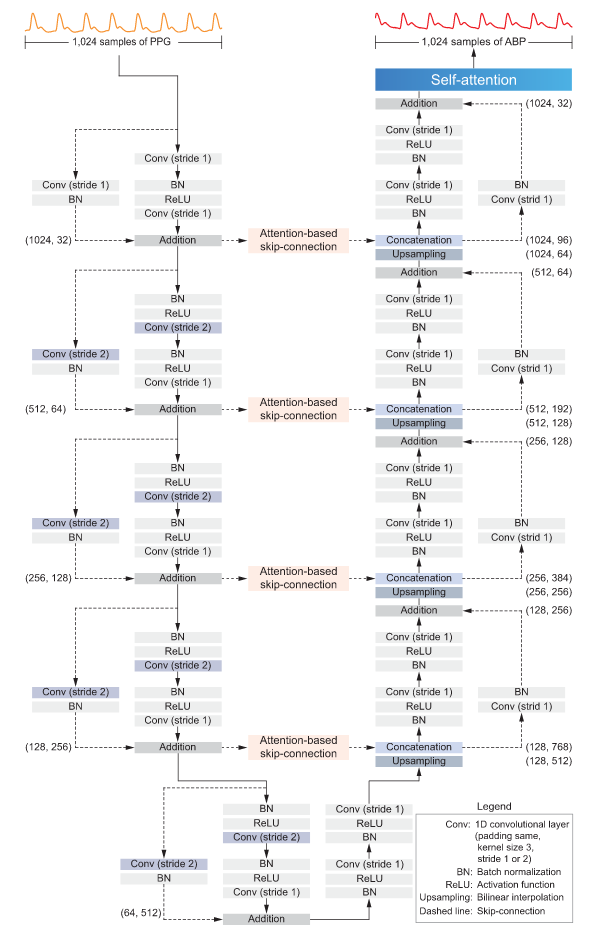
\includegraphics[height=0.4\textheight]{reproductions/kim.png}
        \end{figure}
    \end{columns}

    \begin{table}[htbp]
        \centering
        \resizebox{\linewidth}{!}{
            \begin{tabular}{l SSS SSS}
                \hline
                              & \multicolumn{3}{c}{SBP MAE (mmHg) } & \multicolumn{3}{c}{DBP MAE (mmHg)}                                                                       \\
                \cmidrule(lr){2-4} \cmidrule(lr){5-7}
                Preprocessing & {MLP}                               & {Kim et al. \cite{kim_deepcnap_2022}} & {Imp.} & {MLP}  & {Kim et al. \cite{kim_deepcnap_2022}} & {Imp.} \\
                \hline
                Window        & 22.83                               & 19.1                                  & 3.73   & 12.525 & 12.313                                & 0.212  \\
                Heartbeat     & 18.792                              & 20.701                                & 1.909  & 13.13  & 13.021                                & 0.109  \\
                \hline
            \end{tabular}
        }
    \end{table}

    \begin{itemize}
        \item 145k parameters vs. 5.5B
        \item Complexity doesn't justify the performance Improvement
    \end{itemize}
\end{frame}

\begin{frame}{Contribution 2 \& 3}{Results}
    Overfitting solutions:
    \begin{itemize}
        \item \sout{Increase complexity}
        \item \sout{Increase regularization}
        \item Increase Data
    \end{itemize}
\end{frame}


% Reproduction allows for better comparison
% Large gap between random and patient-wise
% 13.802mmHg lower for random
% Random is generally used in the literature
% Random split passes AAMI doest not generalize
% No models meet AAMI standard for patient-wise

% best patient-wise ais MLP w/ heartbeat sequence
% best overall is RNN-NLP w/ heartbeat sequence
% heartbeat sequence performs the best

% train-test gap random vs patient-wise
% Complexity of model doesn't justify performance Improvement
% OVerfitting, increase complexity(No), increase regularization (no), Increase Data(?)

% Poor dataset variability
